\documentclass[12pt, letterpaper, twoside]{article}
\usepackage[utf8]{inputenc, graphixc, caption, fullpage}
\usepackage[margin=0.5in]{geometry}

\title{APPM 3310: Project Proposal}
\author{Brian Chung}
\author{Seth Hovestol}
\author{Domenic Murtari}
\date{30 October 2015}

\begin{document}

\maketitle

\section{Introduction}

Markov Probability Models are state based conditional directed graphs that
allow predictions on systems where independence cannot be assumed. Graphs can
be represented as matrices, which are where Markov systems gain their power.
We would like to use these methods to analyze the game of Yahtzee in order to
predict the best strategies for fun (and profit).

\section{What is Yahtzee?}

Yahtzee is a game where players roll six-sided dice. After each roll, the
player has the option to roll any number of the five dice again (up to a total
of 3 rolls). Then, the values of the dice are evaluated and scored. For example,
points could be owned for two of a kind, or full house.

This process is continued for 13 rounds. However, the same categories for scoring
cannot be used more than once per game (set of 13 rounds). Finally, the scores
are totaled from each round, with the player with the highest score winning the
game.

\section{Using Markov Models to Analyze Yahtzee}

As Yahtzee revolves around rolling dice, players have an equal chance of
winning the game. Theoretically, victory should be based on luck and not
strategy.

Markov Probability Models are a good fit for analyzing Yahtzee, since each
die can be represented as having six states, ranging from one to six, and also
because each new roll has some transition, whether that be to the same state or
a new state. The probability of each type of set based on the scoring scale will
be used to compare our findings to the values provided by the game of Yahtzee.
Our goal is to examine how closely the point values match with the probability
of rolling a certain patter on dice.

\section{Brief Explanation of Markov Models}

\begin{figure}
  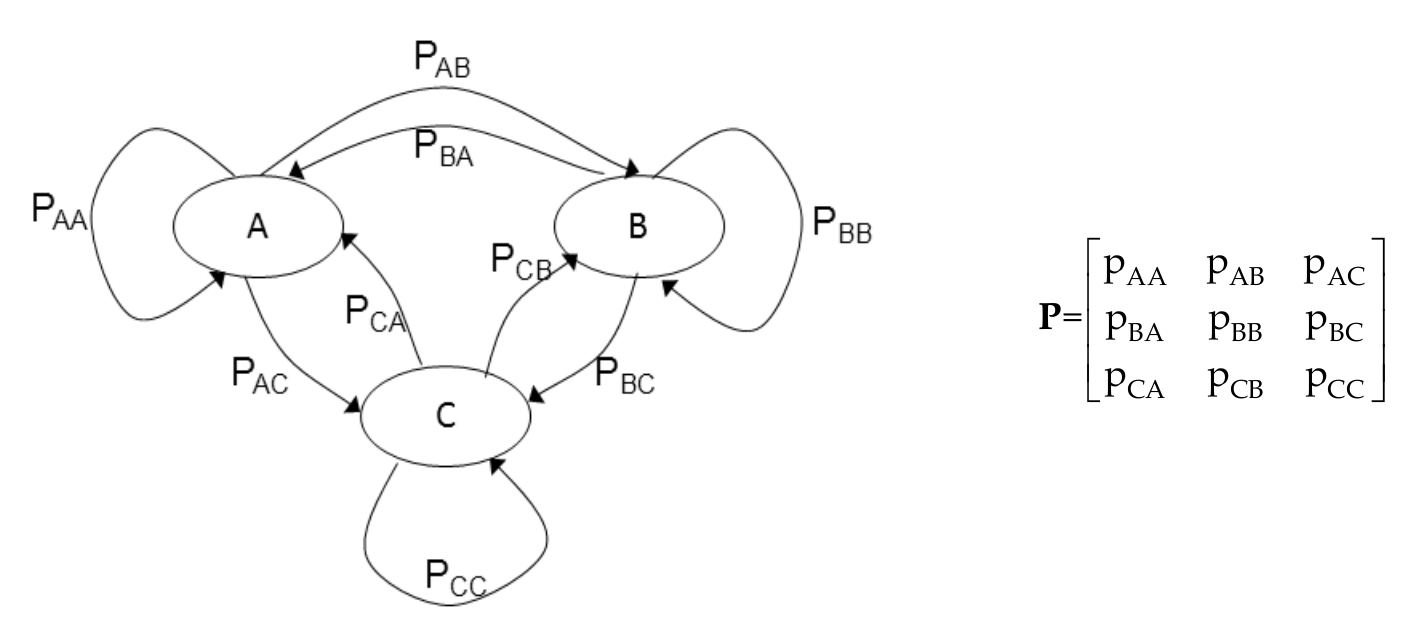
\includegraphics[width=\linewidth]{image11.jpeg}
  \caption[3-State Markov]{Probability transition diagram for a 3-state Markov chain}
  \label{state}
\end{figure}

Because we can use a matrix to represent a directed graph, we can use this matrix
to apply a weight to the edits and predict the outcome of events. Figure 1
shows an example of a graph and the corresponding matrix.\footnote{http://www.intechopen.com/books/matlab-a-fundamental-tool-for-scientific-computing-and-engineering-applications-volume-2/wireless-channel-model-with-markov-chains-using-matlab}

To find the odds of a transition, $P$ can be multiplied by the column vector
$\mathbf{x}=({P_A, P_B, P_C})^T$, where $P_X$ is the probability that the system
is in state $X$. So, $P\mathbf{x}$ results in the probability after one set
of changes, and $P(P\mathbf{x})$ results in the probability after two state
changes. This can be simplified to $P(P\mathbf{x} = (PP)\mathbf{x} = P^2\mathbf{x}$.
This can be further generalized to state that the probability after $n$ state
changes is: $P^n\mathbf{x}$. In the case of Yahtzee, we can use this to optimize
how we play so that we can consistently beat other players.

\section{Wider Applications}

The application of Markov Probability Models are wider than a simple game
of Yahtzee. There are many important applications in fields such as quantum
physics (seen in eigenstates), or any other application where chance plays a
significant role, such as gambling. Understanding the probability of such
situations leads to better approximations and formulations of solutions.

Additionally, knowing the chance of an event can lead to better protection
when the events do not fall within an expected range of events. This can be
seen in coding, where an example may take a few seconds or a few days to
complete depending on conditions. Therefore, knowing the limits of a program
or a solution leads to overall better control of each potential situation.
Situations that arise will be handled in a proper matter, instead of raising
an error.

\end{document}
